\documentclass{article}
\usepackage{graphicx}
\usepackage{booktabs}
\usepackage{amsmath}
\usepackage{geometry}
\usepackage{float}
\geometry{a4paper, margin=1in}

\title{Lab 4: Cache Performance Analysis}
\author{Kaushik Vada}
\date{\today}

\begin{document}

\maketitle

\section{Part 1: Warm-Up (Conceptual Questions)}
\begin{enumerate}
    \item \textbf{Why do modern processors use multiple levels of caches instead of one large cache?} \\
    \textit{Answer:} Processors use a hierarchy (L1, L2, L3) to balance speed and size. A single huge cache would be too slow (high latency), which would bottleneck the CPU. By using a small, super fast L1 cache, the CPU can run at full speed, while the larger L2 and L3 caches catch any misses, so we don't have to go all the way to main memory as often.

    \item \textbf{Define spatial locality and temporal locality. Give one code example of each.} \\
    \textit{Answer:} 
    \textbf{Temporal Locality:} This is when a memory location is accessed and then accessed again really soon (like a loop counter).
    \textbf{Spatial Locality:} This is when we access a memory location and then access nearby locations soon after (like iterating through an array).
    
    \begin{verbatim}
    // Example:
    int sum = 0;
    for (int i = 0; i < 100; i++) {
        sum += A[i]; 
        // 'sum' shows temporal locality (we keep updating it).
        // 'A[i]' shows spatial locality (we go to the next neighbor).
    }
    \end{verbatim}

    \item \textbf{If a cache block is 64 bytes and each int is 4 bytes, how many ints fit in one block?} \\
    \textit{Answer:} Number of integers = $\frac{64 \text{ bytes}}{4 \text{ bytes/int}} = 16 \text{ integers}$.

    \item \textbf{Explain why iterating over a 2D array row-by-row is usually faster than column-by-column.} \\
    \textit{Answer:} In C, 2D arrays are stored in row-major order, so elements in the same row are right next to each other in memory. When we iterate row-by-row, we get good spatial locality: loading one element brings in the whole cache line, so the next few accesses are hits. But if we go column-by-column, we're jumping by a large stride (the row width), which likely causes a cache miss for every single element if the stride is bigger than the cache line.
\end{enumerate}

\section{Part 2: Coding Experiment 1 — Row vs Column Traversal}
We compared the execution time of iterating through a matrix in row-major order versus column-major order for various array sizes ($N \times N$).

\begin{table}[H]
    \centering
    \begin{tabular}{ccc}
        \toprule
        Size (N) & Row-Major Time (s) & Column-Major Time (s) \\
        \midrule
        1024 & 0.002 & 0.006 \\
        2048 & 0.007 & 0.065 \\
        4096 & 0.028 & 0.571 \\
        8192 & 0.111 & 1.546 \\
        \bottomrule
    \end{tabular}
    \caption{Execution time for Row vs Column major access.}
\end{table}

\begin{figure}[H]
    \centering
    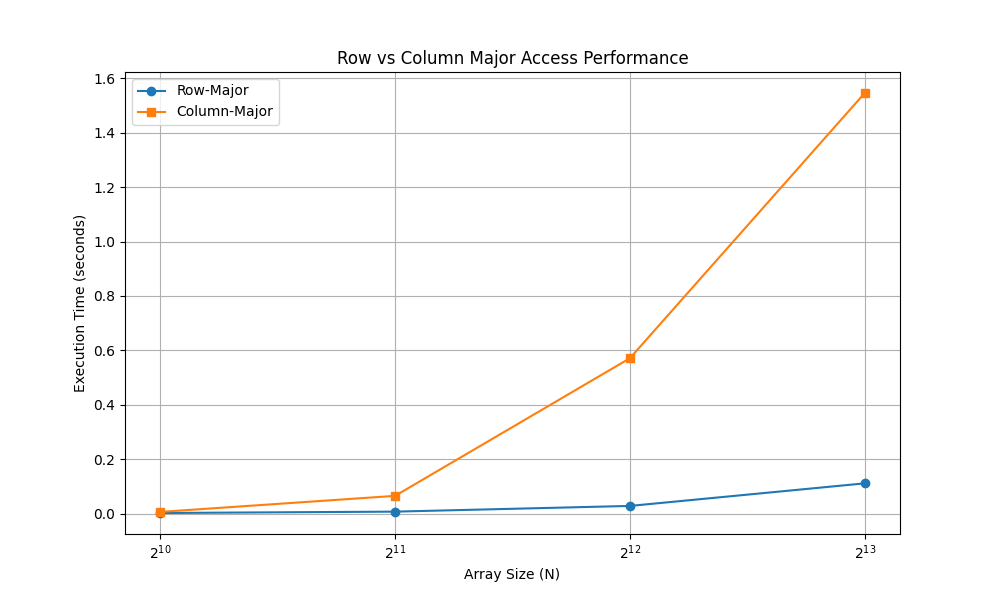
\includegraphics[width=0.8\textwidth]{rowcol_plot.png}
    \caption{Execution Time vs Array Size (Row vs Column Major).}
\end{figure}

\textbf{Analysis:}
Row-major traversal is way faster than column-major traversal for large arrays ($N \ge 1024$). This happens because row-major access uses spatial locality really well—since the data is contiguous, we use the whole cache line. Column-major access, on the other hand, jumps through memory with big strides. Once that stride gets bigger than the cache line, we basically miss the cache on every access, which kills performance.

\section{Part 3: Coding Experiment 2 — Stride Access}
We measured the time to access a 64 MB array with varying stride sizes (powers of 2).

\begin{table}[H]
    \centering
    \begin{tabular}{cc}
        \toprule
        Stride (bytes) & Time (seconds) \\
        \midrule
        4 & 0.023 \\
        8 & 0.028 \\
        16 & 0.042 \\
        32 & 0.069 \\
        64 & 0.174 \\
        128 & 0.227 \\
        256 & 0.381 \\
        512 & 0.228 \\
        1024 & 0.295 \\
        2048 & 0.247 \\
        4096 & 0.280 \\
        8192 & 0.435 \\
        \bottomrule
    \end{tabular}
    \caption{Execution time vs Stride size.}
\end{table}

\begin{figure}[H]
    \centering
    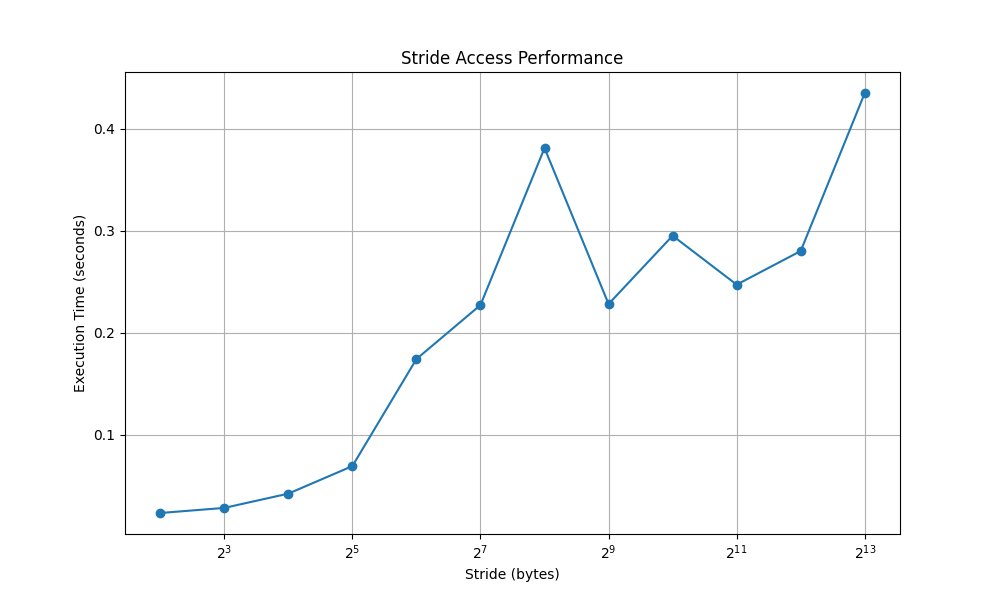
\includegraphics[width=0.8\textwidth]{stride_plot.png}
    \caption{Execution Time vs Stride (Log Scale).}
\end{figure}

\textbf{Analysis:}
As we increased the stride, the execution time went up significantly. There's a huge jump around 64 bytes, which makes sense because that's the typical cache line size. When the stride is small, we get multiple hits per cache line. But once the stride hits 64 bytes, we miss every time. The weird dips and peaks at larger strides (like the dip at 512) are likely due to **cache associativity**. Some strides map to the same sets and cause conflict misses (peaks), while others spread out better or get helped by the prefetcher (dips).

\section{Part 4: Coding Experiment 3 — Matrix Multiply (Naive vs Blocked)}
We compared the performance of naive and blocked matrix multiplication for various matrix sizes ($N$) and block sizes.

\begin{table}[H]
    \centering
    \begin{tabular}{cccc}
        \toprule
        N & Type & Block Size & Time (s) \\
        \midrule
        256 & Naive & - & 0.108 \\
        256 & Blocked & 16 & 0.089 \\
        256 & Blocked & 32 & 0.093 \\
        256 & Blocked & 64 & 0.089 \\
        256 & Blocked & 96 & 0.084 \\
        256 & Blocked & 128 & 0.089 \\
        \midrule
        384 & Naive & - & 0.312 \\
        384 & Blocked & 16 & 0.208 \\
        384 & Blocked & 32 & 0.224 \\
        384 & Blocked & 64 & 0.214 \\
        384 & Blocked & 96 & 0.220 \\
        384 & Blocked & 128 & 0.220 \\
        \midrule
        512 & Naive & - & 0.595 \\
        512 & Blocked & 16 & 0.499 \\
        512 & Blocked & 32 & 0.537 \\
        512 & Blocked & 64 & 0.527 \\
        512 & Blocked & 96 & 0.533 \\
        512 & Blocked & 128 & 0.530 \\
        \bottomrule
    \end{tabular}
    \caption{Matrix Multiplication Performance.}
\end{table}

\begin{figure}[H]
    \centering
    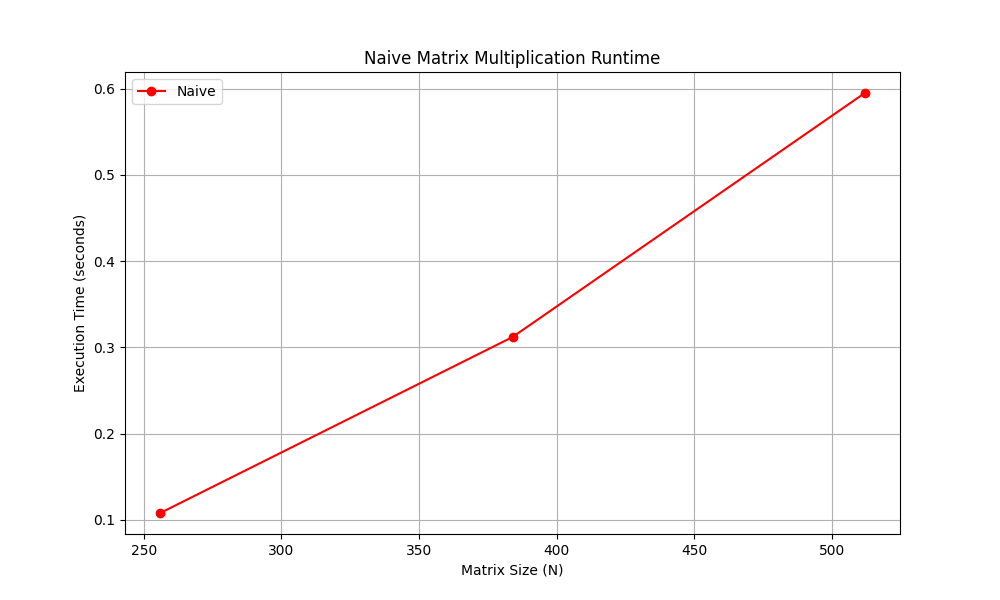
\includegraphics[width=0.8\textwidth]{naive_plot.png}
    \caption{Naive Matrix Multiplication Runtime vs Matrix Size.}
\end{figure}

\begin{figure}[H]
    \centering
    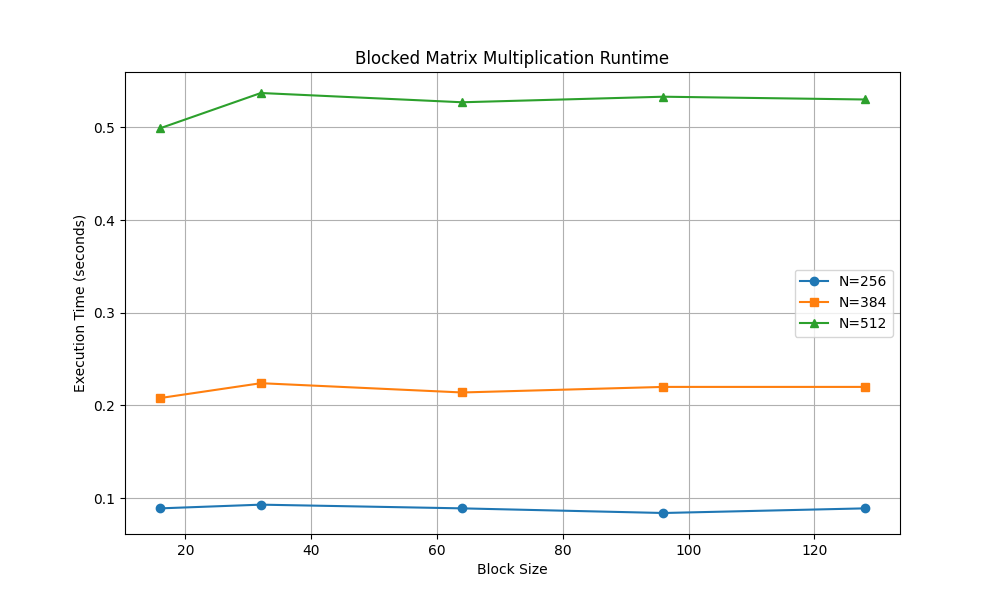
\includegraphics[width=0.8\textwidth]{blocked_plot.png}
    \caption{Blocked Matrix Multiplication Runtime vs Block Size.}
\end{figure}

\textbf{Analysis:}
The blocked matrix multiplication was consistently faster than the naive version. The best block size seems to be around 16 to 96. For the larger matrices (N=512), 16 worked really well. This is because the small blocks fit entirely inside the L1 cache, so we get great temporal locality and don't miss as much. When the blocks get too big, they don't fit in the cache anymore, so performance drops a bit, but it's still better than the naive triple loop.

\section{Conclusion}
In this lab, we saw how important memory access patterns are for performance. Row-major access is much faster because of spatial locality. We also saw that stride access gets way slower once you pass the cache line size. Finally, blocking proved to be a great way to speed up matrix multiplication by keeping data in the cache longer.

\end{document}
